
\documentclass[a4paper,12pt]{article}

\usepackage{inputenc}
\usepackage{euler}
\usepackage[T1]{fontenc}
\usepackage{libertine}
\usepackage{lipsum}
\usepackage{fancyvrb}
\usepackage{url}
\usepackage[english]{babel}
\usepackage{amsmath}
\usepackage{amsthm}
\usepackage{amssymb}
\usepackage{acronym}
\usepackage{hyperref}
\usepackage{tabu}
\usepackage{rotating}
\usepackage{mathdots}
\usepackage{minted}
\usepackage{units}
\usepackage{float}
\usepackage{bbold}
\usepackage[sort&compress,square,comma,authoryear]{natbib}

\fvset{fontsize=\small}
\setmonofont[Scale=0.8]{Menlo}
\usemintedstyle{xcode}
\hypersetup{colorlinks}

\newtheorem{theorem}{Theorem}
\newtheorem{lemma}[theorem]{Lemma}
\newtheorem{proposition}[theorem]{Proposition}
\newtheorem{corollary}[theorem]{Corollary}
\newtheorem{definition}[theorem]{Definition}
\newtheorem{remark}[theorem]{Remark}
\newtheorem{example}[theorem]{Example}

\newcommand{\mycontent}[1]{\textcolor{gray}{#1}}
\newcommand{\zmqfigure}[2]{%
\begin{figure}[H]
\centering
\includegraphics{figures/#1}
\caption{#2}
\end{figure}}

\author{Massimo Nocentini}
\title{ØMQ - The Guide, revisited.}

\begin{document}

\maketitle

\begin{abstract}
ZeroMQ (also known as ØMQ, 0MQ, or zmq) looks like an embeddable networking
library but acts like a concurrency framework. It gives you sockets that carry
atomic messages across various transports like in-process, inter-process, TCP,
and multicast. You can connect sockets N-to-N with patterns like fan-out,
pub-sub, task distribution, and request-reply. It's fast enough to be the
fabric for clustered products. Its asynchronous I/O model gives you scalable
multicore applications, built as asynchronous message-processing tasks. It has
a score of language APIs and runs on most operating systems. ZeroMQ is from
iMatix\footnote{\url{http://www.imatix.com/}} and is LGPLv3 open source.

\mycontent{Our contribution to the official guide \citep{Hintjens:guide} consists in
providing an incomplete set of bindings for Chicken scheme by a minimal and
straightforward translation.}
\end{abstract}

\section*{How It Began}

We took a normal TCP socket, injected it with a mix of radioactive isotopes
stolen from a secret Soviet atomic research project, bombarded it with 1950-era
cosmic rays, and put it into the hands of a drug-addled comic book author with
a badly-disguised fetish for bulging muscles clad in spandex. Yes, ZeroMQ
sockets are the world-saving superheroes of the networking world.
\begin{figure}[H]
\centering
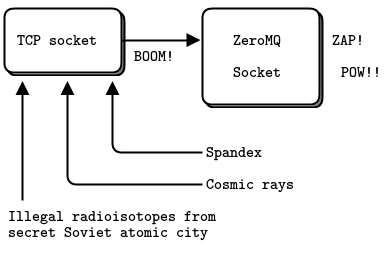
\includegraphics{figures/fig1.png}
\caption{A terrible accident…}
\end{figure}

\section*{The Zen of Zero}

The Ø in ZeroMQ is all about tradeoffs. On the one hand this strange name
lowers ZeroMQ's visibility on Google and Twitter. On the other hand it annoys
the heck out of some Danish folk who write us things like "ØMG røtfl", and "Ø
is not a funny looking zero!" and "Rødgrød med fløde!", which is apparently an
insult that means "may your neighbours be the direct descendants of Grendel!"
Seems like a fair trade.

Originally the zero in ZeroMQ was meant as "zero broker" and (as close to)
"zero latency" (as possible). Since then, it has come to encompass different
goals: zero administration, zero cost, zero waste. More generally, "zero"
refers to the culture of minimalism that permeates the project. We add power by
removing complexity rather than by exposing new
functionality.

\tableofcontents


\section{Basics}

\subsection{Fixing the World}

How to explain ZeroMQ? Some of us start by saying all the wonderful things it
does. It's sockets on steroids. It's like mailboxes with routing. It's fast!
Others try to share their moment of enlightenment, that zap-pow-kaboom satori
paradigm-shift moment when it all became obvious. Things just become simpler.
Complexity goes away. It opens the mind. Others try to explain by comparison.
It's smaller, simpler, but still looks familiar. Personally, I like to remember
why we made ZeroMQ at all, because that's most likely where you, the reader,
still are today.

Programming is science dressed up as art because most of us don't understand
the physics of software and it's rarely, if ever, taught. The physics of
software is not algorithms, data structures, languages and abstractions. These
are just tools we make, use, throw away. The real physics of software is the
physics of people—specifically, our limitations when it comes to complexity,
and our desire to work together to solve large problems in pieces. This is the
science of programming: make building blocks that people can understand and use
easily, and people will work together to solve the very largest problems.

We live in a connected world, and modern software has to navigate this world.
So the building blocks for tomorrow's very largest solutions are connected and
massively parallel. It's not enough for code to be "strong and silent" any
more. Code has to talk to code. Code has to be chatty, sociable,
well-connected. Code has to run like the human brain, trillions of individual
neurons firing off messages to each other, a massively parallel network with no
central control, no single point of failure, yet able to solve immensely
difficult problems. And it's no accident that the future of code looks like the
human brain, because the endpoints of every network are, at some level, human
brains.

If you've done any work with threads, protocols, or networks, you'll realize
this is pretty much impossible. It's a dream. Even connecting a few programs
across a few sockets is plain nasty when you start to handle real life
situations. Trillions? The cost would be unimaginable. Connecting computers is
so difficult that software and services to do this is a multi-billion dollar
business.

So we live in a world where the wiring is years ahead of our ability to use it.
We had a software crisis in the 1980s, when leading software engineers like
Fred Brooks believed there was no "Silver
Bullet"\footnote{\url{http://en.wikipedia.org/wiki/No_Silver_Bullet}} to
"promise even one order of magnitude of improvement in productivity,
reliability, or simplicity".

Brooks missed free and open source software, which solved that crisis, enabling
us to share knowledge efficiently. Today we face another software crisis, but
it's one we don't talk about much. Only the largest, richest firms can afford
to create connected applications. There is a cloud, but it's proprietary. Our
data and our knowledge is disappearing from our personal computers into clouds
that we cannot access and with which we cannot compete. Who owns our social
networks? It is like the mainframe-PC revolution in reverse.

We can leave the political philosophy for another
book\footnote{\url{http://cultureandempire.com/}}. The point is that while the
Internet offers the potential of massively connected code, the reality is that
this is out of reach for most of us, and so large interesting problems (in
health, education, economics, transport, and so on) remain unsolved because
there is no way to connect the code, and thus no way to connect the brains that
could work together to solve these problems.

There have been many attempts to solve the challenge of connected code. There
are thousands of IETF specifications, each solving part of the puzzle. For
application developers, HTTP is perhaps the one solution to have been simple
enough to work, but it arguably makes the problem worse by encouraging
developers and architects to think in terms of big servers and thin, stupid
clients.

So today people are still connecting applications using raw UDP and TCP,
proprietary protocols, HTTP, and Websockets. It remains painful, slow, hard to
scale, and essentially centralized. Distributed P2P architectures are mostly
for play, not work. How many applications use Skype or Bittorrent to exchange
    data?

Which brings us back to the science of programming. To fix the world, we needed
to do two things. One, to solve the general problem of "how to connect any code
to any code, anywhere". Two, to wrap that up in the simplest possible building
blocks that people could understand and use easily.

It sounds ridiculously simple. And maybe it is. That's kind of the whole point.

\subsection{Ask and Ye Shall Receive}

So let's start with some code. We start of course with a Hello World example. We'll make a client and a server. The client sends "Hello" to the server, which replies with "World". Here's the server in C, which opens a ZeroMQ socket on port 5555, reads requests on it, and replies with "World" to each request:
\begin{minted}[baselinestretch=0.8]{c}
//  Hello World server

#include <zmq.h>
#include <stdio.h>
#include <unistd.h>
#include <string.h>
#include <assert.h>

int main (void)
{
    //  Socket to talk to clients
    void *context = zmq_ctx_new ();
    void *responder = zmq_socket (context, ZMQ_REP);
    int rc = zmq_bind (responder, "tcp://*:5555");
    assert (rc == 0);

    while (1) {
        char buffer [10];
        zmq_recv (responder, buffer, 10, 0);
        printf ("Received Hello\n");
        sleep (1);          //  Do some 'work'
        zmq_send (responder, "World", 5, 0);
    }
    return 0;
}
\end{minted}
\mycontent{which is readly translated in Scheme as}
\inputminted[baselinestretch=0.8,stripnl=false]{scheme}{../tests/hello-world/server.scm}
\mycontent{and with little syntactic sugar as}
\inputminted[baselinestretch=0.8,stripnl=false]{scheme}{../tests/hello-world/server-sugar.scm}

\begin{figure}[H]
\centering
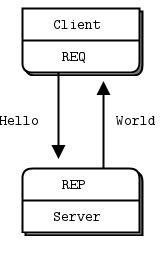
\includegraphics{figures/fig2.png}
\caption{Request-Reply}
\end{figure}
The REQ-REP socket pair is in lockstep. The client issues \Verb|zmq_send()| and
then \Verb|zmq_recv()|, in a loop (or once if that's all it needs). Doing any
other sequence (e.g., sending two messages in a row) will result in a return
code of -1 from the send or recv call. Similarly, the service issues \Verb|zmq_recv()|
and then \Verb|zmq_send()| in that order, as often as it needs to.

Here's the client code:
\begin{minted}[baselinestretch=0.8]{c}
//  Hello World client
#include <zmq.h>
#include <string.h>
#include <stdio.h>
#include <unistd.h>

int main (void)
{
    printf ("Connecting to hello world server…\n");
    void *context = zmq_ctx_new ();
    void *requester = zmq_socket (context, ZMQ_REQ);
    zmq_connect (requester, "tcp://localhost:5555");

    int request_nbr;
    for (request_nbr = 0; request_nbr != 10; request_nbr++) {
        char buffer [10];
        printf ("Sending Hello %d…\n", request_nbr);
        zmq_send (requester, "Hello", 5, 0);
        zmq_recv (requester, buffer, 10, 0);
        printf ("Received World %d\n", request_nbr);
    }
    zmq_close (requester);
    zmq_ctx_destroy (context);
    return 0;
}
\end{minted}
\mycontent{which is readly translated in Scheme as}
\inputminted[baselinestretch=0.8,stripnl=false]{scheme}{../tests/hello-world/client.scm}
\mycontent{and with little syntactic sugar as}
\inputminted[baselinestretch=0.8,stripnl=false]{scheme}{../tests/hello-world/client-sugar.scm}

Now this looks too simple to be realistic, but ZeroMQ sockets have, as we
already learned, superpowers. You could throw thousands of clients at this
server, all at once, and it would continue to work happily and quickly. For
fun, try starting the client and then starting the server, see how it all still
works, then think for a second what this means. \mycontent{It works like a charm}.

Let us explain briefly what these two programs are actually doing. They create
a ZeroMQ context to work with, and a socket. Don't worry what the words mean.
You'll pick it up. The server binds its REP (reply) socket to port 5555. The
server waits for a request in a loop, and responds each time with a reply. The
client sends a request and reads the reply back from the server.

If you kill the server (Ctrl-C) and restart it, the client won't recover
properly. Recovering from crashing processes isn't quite that easy. Making a
reliable request-reply flow is complex enough that we won't cover it until
Section \ref{sec:Reliable:Request:Reply:Patterns}.

There is a lot happening behind the scenes but what matters to us programmers
is how short and sweet the code is, and how often it doesn't crash, even under
a heavy load. This is the request-reply pattern, probably the simplest way to
use ZeroMQ. It maps to RPC and the classic client/server model.

\mycontent{We are developing a component-base approach to define actors and to 
assemble to entire system in a modular way; for the sake of clarity, here are
two augmented versions of clients and servers actors}
\inputminted[baselinestretch=0.8,stripnl=false]{scheme}{../tests/hello-world/hello-world-system-components.scm}
\mycontent{that are collected together in the following system specification}
\inputminted[baselinestretch=0.8,stripnl=false]{scheme}{../tests/hello-world/hello-world-system.scm}
\mycontent{which produces the interaction obtained with the bash command \Verb|tail -f *.out|,}
\VerbatimInput[baselinestretch=0.8]{interaction.out}

\subsection{A Minor Note on Strings}

ZeroMQ doesn't know anything about the data you send except its size in bytes.
That means you are responsible for formatting it safely so that applications
can read it back. Doing this for objects and complex data types is a job for
specialized libraries like Protocol Buffers. But even for strings, you need to
take care.

In C and some other languages, strings are terminated with a null byte. We
could send a string like "HELLO" with that extra null byte:
\begin{minted}[baselinestretch=0.8]{c}
zmq_send (requester, "Hello", 6, 0);
\end{minted}

However, if you send a string from another language, it probably will not
include that null byte. For example, when we send that same string in Python,
we do this:
\begin{minted}[baselinestretch=0.8]{python}
socket.send ("Hello")
\end{minted}

Then what goes onto the wire is a length (one byte for shorter strings) and the
string contents as individual characters.
\zmqfigure{fig3.png}{A ZeroMQ string}
And if you read this from a C program, you will get something that looks like a
string, and might by accident act like a string (if by luck the five bytes find
themselves followed by an innocently lurking null), but isn't a proper string.
When your client and server don't agree on the string format, you will get
weird results.

\textit{When you receive string data from ZeroMQ in C, you simply cannot trust that
it's safely terminated. Every single time you read a string, you should
allocate a new buffer with space for an extra byte, copy the string, and
terminate it properly with a null.}

So let's establish the rule that \textbf{ZeroMQ strings are length-specified and are
sent on the wire without a trailing null}. In the simplest case (and we'll do
this in our examples), a ZeroMQ string maps neatly to a ZeroMQ message frame,
which looks like the above figure—a length and some bytes.

Here is what we need to do, in C, to receive a ZeroMQ string and deliver it to
the application as a valid C string:
\begin{minted}[baselinestretch=0.8]{c}
//  Receive ZeroMQ string from socket and convert into C string
//  Chops string at 255 chars, if it's longer
static char *
s_recv (void *socket) {
    char buffer [256];
    int size = zmq_recv (socket, buffer, 255, 0);
    if (size == -1)
        return NULL;
    if (size > 255)
        size = 255;
    buffer [size] = \0;
    /* use strndup(buffer, sizeof(buffer)-1) in *nix */
    return strdup (buffer);
}
\end{minted}
This makes a handy helper function and in the spirit of making things we can
reuse profitably, let's write a similar \Verb|s_send| function that sends strings in
the correct ZeroMQ format, and package this into a header file we can reuse.

The result is \Verb|zhelpers.h|, \mycontent{whose partial porting is shown in Section 
\ref{sec:zhelpers:scm}}, which lets us write sweeter and shorter ZeroMQ
applications in C. It is a fairly long source, and only fun for C developers,
so read it at leisure\footnote{\url{https://github.com/imatix/zguide/blob/master/examples/C/zhelpers.h}}.

\subsection{Version reporting}

ZeroMQ does come in several versions and quite often, if you hit a problem,
it'll be something that's been fixed in a later version. So it's a useful trick
to know exactly what version of ZeroMQ you're actually linking with.

Here is a tiny program that does that:
\begin{minted}[baselinestretch=0.8]{c}
//  Report 0MQ version

#include <zmq.h>

int main (void)
{
    int major, minor, patch;
    zmq_version (&major, &minor, &patch);
    printf ("Current 0MQ version is %d.%d.%d\n", major, minor, patch);
    return 0;
}
\end{minted}
\mycontent{which is readly translated as}
\inputminted[baselinestretch=0.8,stripnl=false]{scheme}{../tests/version/version.scm}
\mycontent{so that it prints to the stdout port \Verb|(Current ∅MQ version is (4 3 1))|.}

\subsection{Getting the Message Out}

The second classic pattern is one-way data distribution, in which a server
pushes updates to a set of clients. Let's see an example that pushes out
weather updates consisting of a zip code, temperature, and relative humidity.
We'll generate random values, just like the real weather stations do.

Here's the server. We'll use port 5556 for this application:
\begin{minted}[baselinestretch=0.8]{c}
//  Weather update server
//  Binds PUB socket to tcp://*:5556
//  Publishes random weather updates

#include "zhelpers.h"

int main (void)
{
    //  Prepare our context and publisher
    void *context = zmq_ctx_new ();
    void *publisher = zmq_socket (context, ZMQ_PUB);
    int rc = zmq_bind (publisher, "tcp://*:5556");
    assert (rc == 0);

    //  Initialize random number generator
    srandom ((unsigned) time (NULL));
    while (1) {
        //  Get values that will fool the boss
        int zipcode, temperature, relhumidity;
        zipcode     = randof (100000);
        temperature = randof (215) - 80;
        relhumidity = randof (50) + 10;

        //  Send message to all subscribers
        char update [20];
        sprintf (update, "%05d %d %d", zipcode, temperature, relhumidity);
        s_send (publisher, update);
    }
    zmq_close (publisher);
    zmq_ctx_destroy (context);
    return 0;
}
\end{minted}
There's no start and no end to this stream of updates, it's like a never ending
broadcast. \mycontent{The translation is in order:}
\inputminted[baselinestretch=0.8,stripnl=false]{scheme}{../tests/publish-subscribe/server.scm}
\mycontent{together with the syntactic sugar,}
\inputminted[baselinestretch=0.8,stripnl=false]{scheme}{../tests/publish-subscribe/server-sugar.scm}

Here is the client application, which listens to the stream of updates and
grabs anything to do with a specified zip code, by default New York City
because that's a great place to start any adventure:
\begin{minted}[baselinestretch=0.8]{c}
//  Weather update client
//  Connects SUB socket to tcp://localhost:5556
//  Collects weather updates and finds avg temp in zipcode

#include "zhelpers.h"

int main (int argc, char *argv [])
{
    //  Socket to talk to server
    printf ("Collecting updates from weather server…\n");
    void *context = zmq_ctx_new ();
    void *subscriber = zmq_socket (context, ZMQ_SUB);
    int rc = zmq_connect (subscriber, "tcp://localhost:5556");
    assert (rc == 0);

    //  Subscribe to zipcode, default is NYC, 10001
    char *filter = (argc > 1)? argv [1]: "10001 ";
    rc = zmq_setsockopt (subscriber, ZMQ_SUBSCRIBE,
                         filter, strlen (filter));
    assert (rc == 0);

    //  Process 100 updates
    int update_nbr;
    long total_temp = 0;
    for (update_nbr = 0; update_nbr < 100; update_nbr++) {
        char *string = s_recv (subscriber);

        int zipcode, temperature, relhumidity;
        sscanf (string, "%d %d %d",
            &zipcode, &temperature, &relhumidity);
        total_temp += temperature;
        free (string);
    }
    printf ("Average temperature for zipcode '%s' was %dF\n",
        filter, (int) (total_temp / update_nbr));

    zmq_close (subscriber);
    zmq_ctx_destroy (context);
    return 0;
}
\end{minted}
\mycontent{Again, the translation is in order:}
\inputminted[baselinestretch=0.8,stripnl=false]{scheme}{../tests/publish-subscribe/client.scm}
\mycontent{together with the syntactic sugar,}
\inputminted[baselinestretch=0.8,stripnl=false]{scheme}{../tests/publish-subscribe/client-sugar.scm}

\mycontent{A corresponding components definition is,}
\inputminted[baselinestretch=0.8,stripnl=false]{scheme}{../tests/publish-subscribe/pub-sub-system-components.scm}
\mycontent{and the whole system specification,}
\inputminted[baselinestretch=0.8,stripnl=false]{scheme}{../tests/publish-subscribe/pub-sub-system.scm}
\mycontent{together yield the interaction}
\VerbatimInput[baselinestretch=0.8]{pub-sub-interaction.out}

\zmqfigure{fig4.png}{Publish-Subscribe}
Note that when you use a SUB socket you must set a subscription using
\Verb|zmq_setsockopt()| and SUBSCRIBE, as in this code. If you don't set any
subscription, you won't get any messages. It's a common mistake for beginners.
The subscriber can set many subscriptions, which are added together. That is,
if an update matches ANY subscription, the subscriber receives it. The
    subscriber can also cancel specific subscriptions. A subscription is often,
    but not necessarily a printable string. See
    \Verb|zmq_setsockopt()|\footnote{\url{http://api.zeromq.org/3-2:zmq\_setsockopt}}
    for how this works.






\section{Reliable Request-Reply Patterns}
\label{sec:Reliable:Request:Reply:Patterns}

\section{Appendix}

\subsection{\texttt{zmq.scm}}
\inputminted[baselinestretch=0.8,stripnl=false]{scheme}{../src/zmq.scm}

\subsection{\texttt{zhelpers.scm}}
\label{sec:zhelpers:scm}
\inputminted[baselinestretch=0.8,stripnl=false]{scheme}{../src/zhelpers.scm}

\subsection{\texttt{zsugar.scm}}
\inputminted[baselinestretch=0.8,stripnl=false]{scheme}{../src/zsugar.scm}


\bibliographystyle{plainnat}
\bibliography{biblio}
\end{document}
